\documentclass[10pt,a4paper,final,oneside,openany]{memoir}

\usepackage[english]{babel}
\usepackage[utf8]{inputenc}
\usepackage[T1]{fontenc}
\usepackage[british]{isodate}

% Layout Fixes
\usepackage{booktabs} % nicer spacing between table rulers
\usepackage{microtype}
\usepackage{fixltx2e} % To prevent the figures from being placed
                      % out-of-order with respect to their
                      % "non-starred" counterparts


\usepackage{amsmath,amssymb, amsbsy}
\usepackage[amsmath,amsthm,thmmarks]{ntheorem}
\usepackage{semantic, stmaryrd}
\usepackage{graphicx}
\usepackage{todonotes}
\presetkeys{todonotes}{inline}{}
\usepackage{adjustbox}
\usepackage{tikz}
\usetikzlibrary{trees}
\usepackage{algpseudocode}
\usepackage{algorithm}
\usepackage{listings}

\lstset{basicstyle=\footnotesize\ttfamily,breaklines=true, language=Haskell}

% ADD "parfor" to algorithmic environment
  % declaration of the new block
  \algblock{ParFor}{EndParFor}
  % customising the new block
  \algnewcommand\algorithmicparfor{\textbf{parfor}}
  \algnewcommand\algorithmicpardo{\textbf{do}}
  \algnewcommand\algorithmicendparfor{\textbf{end\ parfor}}
  \algrenewtext{ParFor}[1]{\algorithmicparfor\ #1\ \algorithmicpardo}
  \algrenewtext{EndParFor}{\algorithmicendparfor}

% Bibliography
%\usepackage[style=alphabetic,natbib=true]{biblatex}
\usepackage[hyperref,style=numeric,natbib=true, defernumbers=true]{biblatex}
\usepackage[hyperindex,hidelinks]{hyperref}

% Fonts
\usepackage{palatino}
\linespread{1.05}
\usepackage[scaled]{beramono}

% customize chapter pages
\makepagestyle{myheadings}
\makepagestyle{myheadingschapterpage}
\makeevenfoot{myheadingschapterpage}{}{\thepage}{}
\makeoddfoot{myheadingschapterpage}{}{\thepage}{}
\aliaspagestyle{chapter}{myheadingschapterpage}
\aliaspagestyle{title}{myheadingschapterpage}
\makeevenhead{myheadings}{}{\scshape \thetitle}{}
\makeoddhead{myheadings}{}{\footnotesize\scshape \thetitle}{}
\makeevenfoot{myheadings}{}{\thepage}{}
\makeoddfoot{myheadings}{}{\thepage}{}
\pagestyle{myheadings}

\def\thefigure{\arabic{figure}}
\setcounter{tocdepth}{0}


\setcounter{secnumdepth}{1}
\setcounter{chapter}{0}
\setsecheadstyle{\large\bfseries\raggedright}
\setsubsecheadstyle{\bfseries}

% BIBLIOGRAPHY styling
% Print the DOI url out
%\newcommand*{\doi}[1]{DOI: \url{http://dx.doi.org/#1}}

\DeclareFieldFormat{doi}{\textsc{doi}: \url{http://dx.doi.org/#1}}
\DeclareNameAlias{default}{last-first/first-last}
%\DeclareFieldFormat{title}{\emph{#1}}
\renewcommand\mkbibnamefirst[1]{\textsc{#1}}
\renewcommand\mkbibnamelast[1]{\textsc{#1}}
\renewcommand*{\bibfont}{\footnotesize}

% No page numbers for parts in TOC
\cftpagenumbersoff{part}
% Footnote symbols
%\renewcommand*{\thefootnote}{\fnsymbol{footnote}}

% Figures
\newsubfloat{figure}

\usepackage{sidecap}
\usepackage{caption}
\captionsetup{margin=0pt, font=small, labelfont=bf, format=hang}
\setlength{\abovecaptionskip}{0pt}
\setlength{\belowcaptionskip}{0pt}


% Default commands
\newcommand{\subimgwidth}{.48\textwidth}
\newcommand{\imgwidth}{.85\textwidth}


\newtheorem{example}{Example}
%
\theoremstyle{plain}
\theoremsymbol{\tiny $\Box$}
\newtheorem{definition}[equation]{Definition}






%%% Local Variables: 
%%% mode: latex
%%% TeX-master: "master"
%%% End: 


\title{Applying functional data-parallel languages to option pricing}
\author{
  Martin Dybdal -- \texttt{dybber@dybber.dk} \\
  Philip Carlsen -- \texttt{plcplc@gmail.com}
\\
University of Copenhagen, DIKU}

\date{March 2013}

\bibliography{../bibliography/bibliography}

% Write "Part II" etc. in TOC instead of just "II"
\renewcommand*{\cftpartname}{Part\space}

\begin{document}
\frontmatter

% % Center title page
% \begin{titlingpage}
%   \calccentering{\unitlength} % forudsat \unitlength ikke bruges til andet
%   \begin{adjustwidth*}{\unitlength}{-\unitlength}
%   \begin{adjustwidth}{-1cm}{-1cm}

%   \maketitle

%   \begin{abstract}
%     This abstract is intentionally left blank
%   \end{abstract}

%   \end{adjustwidth}
%   \end{adjustwidth*}
% \end{titlingpage}

\includepdf{coverpage/coverpage}
% ~  ~\thispagestyle{empty}
 \clearpage
~
\vspace{3cm}
  \begin{abstract}
    We evaluate the current state of functional data-parallel
    languages through the implementation of option pricing
    algorithms. Specifically, we implement a lattice-based binomial
    option pricer \cite{cox1979option}, the least-squares Monte Carlo
    algorithm \cite{longstaff2001valuing}, and a Sobol sequence
    generator \cite{bratley1988algorithm}.

    Motivated by our attempts at implementing these algorithms, we
    identify that both Nikola \cite{mainland2010nikola}, Accelerate
    \cite{chakravarty2011accelerating} and the Haskell library Repa
    \cite{keller2010regular} lack support for iterative array
    construction. We suggest the addition of new constructs and
    present possible implementation strategies.

    We demonstrate a lack of composability in the current languages,
    caused by imposed limitations that forbid nested array
    operations. This suggests that the problem of compiling nested
    parallel operations should be addressed rather than avoided.

    The currently most popular approach to compilation of irregular
    nested data-parallel languages is the vectorisation
    transformation, as implemented in NESL \cite{nesl} and Data
    Parallel Haskell \cite{spj2008dph}. \todo{mention Copperhead} We
    suggest an alternative approach for regular nested
    data-parallelism, which relies on a cursor to mark the division
    between parallel and sequential code, much inspired by similar
    constructs found in Repa. The approach allows for experimentation
    with parallelisation strategies and our proposal could lead to a
    language for heterogeneous computing.
  \end{abstract}

% \clearpage
%  ~\thispagestyle{empty}
\clearpage
\tableofcontents*
%\openany
\chapter{Preface}
This dissertation is submitted in fulfilment of the graduate education
in computer science (\textit{datalogy}) at the University of
Copenhagen, for Philip L. Carlsen and Martin Dybdal. In addition, the
dissertation also serves as partial fulfilment of Martin Dybdal's 4+4
Ph.D. education at the University of Copenhagen.

The thesis has been supervised by Ken Friis Larsen and we would like
to thank him for valuable supervision hours .... We would also like to
thank Geoffrey Mainland and Trevor McDonell for valuable email
correspondences and quick responses in cases of problems with their
libraries... Finally we would like to thank Cosmin Oancea, Christian
Andretta, Jost Berthold, Martin Elsman and others here at the HIPERFIT
research center.

%\openright
\mainmatter
\counterwithout{table}{chapter}
\counterwithout{figure}{chapter}
\chapter{Introduction}
\begin{itemize}
\item The free lunch is over
\item Areas where high-performance computing is found fruitful
\item Embarassingly parallel problems
\item Why the language-based approach?
\item Parallel Functional Programming
\item What is a "vector language"?
\end{itemize}

\section{Report outline}
The report is structured as follows. This introductory chapter is
supplemented with two terminology introducing chapters, one on the
financial example problems we are going to use throughout the report
and one on hardware platforms such as GPUs. The rest of the report
after these introductory chapters is divided into two independent
parts. The first part contains a survey of currently used vector
languages and their implementation techniques. The second part
describes our own efforts into \ldots

%%% Local Variables: 
%%% mode: latex
%%% TeX-master: "master"
%%% End: 

\chapter{General-purpose programming of GPUs}
\label{chap:gpgpu}
Graphics processing units (GPUs) show a high degree of data
parallelism, originating from their \textit{single instruction,
  multiple data}-architecture (SIMD), where a set of processor cores
executes the same program in lock-step on each their own data
item. Many tasks in scientific computing and engineering, such as
simulation or genome pattern matching, are data-parallel in
nature. For instance, when simulating physical systems, there are
often many millions of interacting agents (e.g. reacting atoms in
chemistry) that can be updated independently in each step of the
simulation. In other cases we might want to run the same simulation
thousands of times and average the outcomes.

Originally, the only programming interfaces for GPUs were based on
concepts from computer graphics, such as textures and shader
programs. Applications outside the domain of computer graphics had to
be encoded to fit the models of programming interfaces such as OpenGL
or DirectX and developers needed deep knowledge about the
GPU-architecture \cite{nvidia2009fermi}. Since scientists started to
use GPUs for research projects, several programming frameworks have
been developed. The two most prominent and widely used today are
OpenCL and CUDA.

In this chapter we will look at the architecture of a modern NVIDIA
GPU and the programming model of NVIDIA's CUDA framework. The chapter
is an edited version of a text on GPUs previously produced by one of
the authors (see \cite{dybdal2011opencl}).

\section{GPU hardware}
\label{sec:gpu_hardware}
The execution of a GPU program has to be conducted by an accompanying
program executing on the CPU. The traditional CPU is referred to as
the \textit{host} and the GPU is called the \textit{device}. Other
concepts such as pointers or arrays are often prefixed with either of
these to specify where they reside.

A CUDA device is divided into a number of \textit{streaming
  multiprocessors} (SMs), each of which are in turn divided into
individual CUDA cores. It is these CUDA cores that performs the actual
computation on a GPU. How these concepts are related is shown in
Figure \ref{fig:gpu_terminology}, together with the three
corresponding layers of GPU-memory and communication pathways. Each
CUDA core has an amount of register space available, which are memory
local to the current thread executing on that core. To communicate and
synchronize between other threads, each streaming multiprocessor
provides an amount of shared memory, which are a bit slower than
registers. As a last layer, the GPU provides a large amount of global
memory, shared between all SMs, with the drawback of very long access
times.

\begin{figure*}
  \centering
  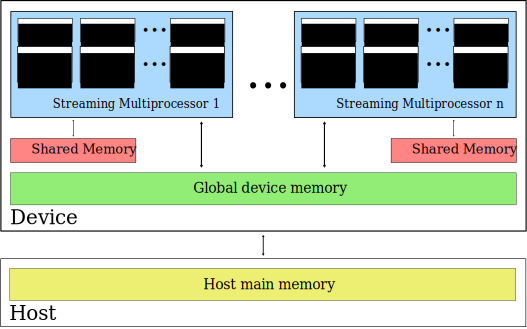
\includegraphics[width=\textwidth]{graphics/cuda-structure}
  \caption{CUDA GPU terminology: Host, devices, streaming
    multiprocessors and CUDA cores. The arrows show the possible path
    of data movement. The host can command movement of data to and
    from host memory and device memory. Kernel code is responsible for
    moving data between global memory, shared memory and registers.}
  \label{fig:gpu_terminology}
\end{figure*}

The architecture of NVIDIAs latest line of GPGPU devices is named
Kepler. The current Kepler based GPUs consists of up to 2880 CUDA
cores grouped into streaming multiprocessors of 192 cores each
\cite{nvidia2012keplerGK110}. At the HIPERFIT Research Center we have
access to a machine with two GeForce GTX 690 GPUs, each of which
contains two Kepler GK104 GPUs. The Kepler GK104 GPU is equipped with
1536 CUDA cores arranged into eight multiprocessors and shared between
all SMs is an L2 Cache (512 KB) and 2 GiB global memory
\cite{nvidia2012geforcegtx680}.

Figure \ref{fig:kepler_sm} shows the structure of a Kepler GK104
streaming multiprocessor. All 192 cores share the same register file
and 64 KB of additional memory which can be used both as L1 cache and
shared memory between for the CUDA cores of the SM. The amount of
memory used as cache and as shared memory is configurable.

\begin{figure}
  \centering
  \includegraphics[width=0.8\textwidth]{graphics/nvidia_kepler_gk104_sm_cropped}
  \vspace{2mm}
  \caption{A diagram of a single streaming multiprocessor from a
    Kepler GK104 GPU. The illustration is borrowed from NVIDIAs GK104
    whitepaper \cite{nvidia2012geforcegtx680}, and a few irrelevant
    parts are cropped away..}
  \label{fig:kepler_sm}
\end{figure}

\section{GPU programming}
Since modern GPUs contains hundreds or thousands of cores, GPU
programs must be written such that their work can be executed
independently and in parallel on as many cores as possible. A single
thread of execution on a CUDA core is the smallest unit of work on a
GPU and programming a GPU is done by writing \textit{kernel programs}
or simply \textit{kernels}, which specifies the work done by a single
thread.

These threads are arranged into equal sized groups called
\textit{blocks} and blocks are arranged into a grid.  It is the task
of kernel program itself to find the subset of the data that it has
to work on. That is, all executions of the kernel receives exactly the
same arguments, but the kernel can query where it is located in its
block and where that block is located in the grid, to determine which
part of the input arrays to work on.

When executing a grid of CUDA blocks on a Kepler architecture GPU,
each block is assigned to a single SM (each SM can process several
blocks). Each block is partitioned into \textit{warps} which are
groups of 32 threads, which are scheduled on the 192 CUDA cores of the
streaming multiprocessor. % \todo{explain warp schedulers and why there
  % are 4 rather than 6 schedulers}

All threads in a \textit{warp} always executes exactly the same
instruction, this is called \textit{SIMD}, single instruction,
multiple data. Moreover, when warps are executed by a SM it can
execute two warps from the same block simultaneously, as each SM have
access to two schedulers and the register file can be used for both of
the two warps independently. This is called \textit{SIMT} (single
instruction, multiple thread) as two threads are executed on the same
processor simultaneously. Each streaming multiprocessor can be
assigned a certain number of warps, which it switches between
executing. This is useful for hiding latency endured by memory access
or data dependencies between instructions.

\subsection{Synchronization}
It is not uncommon that several threads has to interact, when they are
cooperating to solve a problem. In these cases synchronization
primitives are necessary to avoid race-conditions. In CUDA there are
two levels of inter-thread synchronization. A kernel can synchronize
with the rest of the threads in its block by calling the
\lstinline{__syncthreads} CUDA function. To synchronize across blocks,
the programmer has to split program into two independent kernels and
call them sequentially with a call to \lstinline{cudaDeviceSynchronize}
in between.

\subsection{Optimization considerations}
Determining how the grid of threads are partitioned into blocks are of
importance when optimizing for fast execution. There should at least
be as many blocks as there are streaming multiprocessor, to avoid
having a stalled processor. If blocks have to wait for synchronization
with other blocks it might also be beneficial to have more than one
block per SM.

The size of blocks should also be considered, as having enough
available warps can hide latency from memory transactions. Accessing
global memory can stall a streaming multiprocessor for 200-400 cycles,
where as local memory access only partakes a couple of cycles
\cite{nvidia2012cudaguide}. This is not the largest bottleneck though,
as GPUs are presently connected to the host through PCI Express ports
which have a throughput limit of a little under 8 GB/s (with PCI
Express 3.0). Accessing global memory on the device can be done at
192.3 GB/s, for the GeForce GTX 690 (and the double of that if you
count both of its GPUs).

We just argued for increasing block size, to make sure there are
enough warps, but it is not always good for efficiency to have large
blocks, as each streaming multiprocessor has a limited amount of
registers and local memory. All threads currently executed on a SM
shares the same register-file, and blocks are only assigned to a SM if
there are enough available registers for all of its threads. Thus, to
get optimal occupancy, blocks must be sized such that the size of the
register-file is divisible by the total amount of needed registers. An
occupancy calculator created by NVIDIA is available as a spreadsheet
on the NVIDIA
website\footnote{\url{http://developer.download.nvidia.com/compute/cuda/CUDA_Occupancy_calculator.xls}}.

\subsection{Memory access patterns}
Accessing global device memory is always done in segments of 32, 64 or
128 bytes, and these accesses must be aligned such that segments are
placed in physical device memory with a segment, starting on addresses
that are a multiple of the segment size
\cite{nvidia2012cudaguide}. When a warp gets executed, the memory
transaction of individual threads are coalesced such that the needed
memory can be fetched by a single memory transaction. To minimize the
number of memory transactions, it is thus important to write kernels,
such that nearby threads which are scheduled in the same warp, will
access memory in the same memory region. Previous architectures had
strict rules for how data accesses should be distributed. If
simultaneous operations on memory from a warp was out of sequence on
such a device, all the operations was performed as separate memory
transactions. The same would happen if accesses were not aligned
correctly. From Compute Capability 2.X and higher, the global L2 Cache
is used, such that out of order accesses can be coalesced into single
transactions and misalignments can be handled as long as they do not
cross 128 byte boundaries. If a segment of 32 bytes are accessed such
that this access overlap two physical 32-byte segments, the 64-byte
segment containing both of them are loaded from global memory instead.

These considerations are explained in detail in ``The CUDA C
Programming Guide'' by NVIDIA \cite[Section~5.3.2]{nvidia2012cudaguide}.

%%% Local Variables:
%%% mode: latex
%%% TeX-master: "master"
%%% End:

\chapter{Cases}

In this chapter we will introduce the cases from which we take our offset in
our contributions. As we are motivated by financial problems, our cases are
drawn from that domain and the surrounding domain of scientific computing in
general.

\section{The binomial option pricing model}
\label{sec:binomial-model}
A relatively simple discrete time model for computing the price of an
American style option is the \emph{standard binomial model}
\cite{cox1979option}. The model is widely used in the financial
industry \cite{ganesan2009acceleration}, and is thus a relevant case
for our investigation.

The basic assumption is that the price of the underlying follows a
binomial process over equally spaced time steps. This makes it
possible to write out the possible future states of the
underlying. Moving a single time step forward, the binomial process
produces two possible future states of the underlying. The value of
the underlying can go either up or down with probabilities $q$ and $1
- q$ respectively. We denote the rate of up and down movement as $u$
and $d$ respectively. The change over one period $\Delta t$ is thus
given as:

$$S(t+\Delta t) = \left\{
  \begin{array}{ll}
    S(t)u & \quad \text{with probability $q$} \\
    S(t)d & \quad \text{with probability $1-q$}
  \end{array} \right.
$$

We skip the discussion of how to compute the constants $q$, $u$ and
$d$ and refer to the paper by Cox, Ross and Rubinstein that introduced
the model \cite{cox1979option}. After several time steps the binomial
process will unfold into a lattice of possible futures states as shown
in Figure \ref{fig:binomial-tree}. In this example we have assumed
that $u$ and $d$ has been selected such that $u\cdot d = 1$, but that
is not a necessity.

\begin{figure}
  \centering
  \tikzstyle{nodestyle} = [text centered, minimum size=0.42cm, inner sep=0]

\begin{tikzpicture}
  \node at (0,0) [nodestyle] (S1) {$S(t_0)$};

  \node at (-1, -1) [nodestyle] (dS) {$dS(t_0)$};
  \node at ( 1, -1) [nodestyle] (uS) {$uS(t_0)$};

  \node at ( 2, -2) [nodestyle] (u2S) {$u^2S(t_0)$};
  \node at ( 0, -2) [nodestyle] (S2) {$S(t_0)$};
  \node at (-2, -2) [nodestyle] (d2S) {$d^2S(t_0)$};

  \node at ( 3, -3) [nodestyle] (u3S) {$u^3S(t_0)$};
  \node at ( 1, -3) [nodestyle] (uS2) {$uS(t_0)$};
  \node at (-1, -3) [nodestyle] (dS2) {$dS(t_0)$};
  \node at (-3, -3) [nodestyle] (d3S) {$d^3S(t_0)$};

  \node at (-4.5,  0) [] (t0) {$S(t_0) =$};
  \node at (-4.5, -1) [] (t0) {$S(t_1) =$};
  \node at (-4.5, -2) [] (t0) {$S(t_2) =$};
  \node at (-4.5, -3) [] (t0) {$S(t_3) =$};

  \path[-latex]
     (S1) edge (uS)
     (S1) edge (dS)

     (uS) edge (S2)
     (dS) edge (S2)
     (uS) edge (u2S)
     (dS) edge (d2S)

     (u2S) edge (u3S)
     (u2S) edge (uS2)
     (S2)  edge (uS2)
     (S2)  edge (dS2)
     (d2S) edge (dS2)
     (d2S) edge (d3S);
\end{tikzpicture}

\vspace{2mm}

\caption{Lattice generated by the binomial process of a single
  underlying over three periods ($T=t_3$). The root
  node represents the current price of the underlying and the leafs
  represents possible values at expiration time.}
\label{fig:binomial-tree}
\end{figure}

Each layer in the tree corresponds to a time step $t$, and the nodes
of the layer are the different possible prices $S(t)$ of the
underlying. To distinguish between the nodes on a single layer we
attach a unique index $i$ to each node of the tree and define
$\mathsf{left\textsf{-}child}(i)$ and
$\mathsf{right\textsf{-}child}(i)$ to navigate the indices of the
tree. We use the notation $S_i(t)$ to refer to the particular node $i$
at layer $t$.

The final row represents the possible values of the underlying at
expiration time, $T$. We can use the same procedure as for European
options (discussed in Example \ref{example:europeancall} above) to
find the value of our option at each of these possible cases. Thus,
for each possible $S_i(T)$, that is, for each leaf node, we compute
the option value as either $V_i(T) = max(S_i(T)-K, 0)$ for call
options or $V_i(T) = max(K-S_i(T),0)$ for put options, where $K$ is
the strike price.

The algorithm now proceeds by estimating the price $V_i$ of the option
in the remaining lattice points, by iterating backwards (towards the
root). The price estimate at each lattice point for time $t$ depends
only on its two children at time $t+1$, which prices was calculated in
the previous iteration. This is done by recursively discounting:
$$V_{i} = e^{-r\Delta t} \cdot (q\cdot V_{\mathsf{left\textsf{-}child}(i)} + (1-q)\cdot V_{\mathsf{right\textsf{-}child}(i)})$$
where the probability $q$ is used to attain the expected value from
either of the two alternative futures, and $e^{r\Delta t}$ is the
guaranteed scale of increment over a single time period $\Delta t$ for
a riskless investment with interest rate $r$.

% \todo{Display the full binomial algorithm and parameters in a concise fact-box
% like format. Be sure to explain what $S(i,t)$ is.}

% In equations, this may be written as follows, where $x_{i,t}$ represents a
% lattice point.

% \begin{align*}
% v(x_{i,t}) &= h(f_{i,t}(v(x_{i,t+1})),g_{i,t}(v(x_{i+1,t+1}))) \\
% v(x_{i,T}) &= \max\{ 0, k - S(i,T) \} \tag{for a put-option}\\
% v(x_{i,T}) &= \max\{ 0, S(i,T) - k \} \tag{for a call-option}\\
% \end{align*}

% In our case the functions $f_{i,t},g_{i,t},h$ contain only simple constant-time
% arithmetic calculation.

\subsection{Implementation Techniques}
As seen above, the value of $V_i(t)$ depends only on values associated
with time $t+1$. Therefore, for each $t$, the evaluation of $V_i(t)$'s may
proceed in parallel.

Algorithm \ref{alg:binomial-algorithm} illustrates this in pseudocode
that uses only two arrays in tandem to hold the intermediately
produced values. It should also be observed that it is not necessary
to build the complete lattice, as we are only interested in the values
at expiration date.

\begin{algorithm}
% \begin{verbatim}
% binom:
%   -- A,B are assumed preallocated, and T is assumed odd.
%   t <- T
%   B <- parmap (\i -> max 0 (k-S(i,T))) [0..T]
%   while t > 0
%     A <- parmap (\i -> h(f_{i,t}(B[i]),g_{i,t}(B[i+1))) [0..t]
%     t <- t -1
%     B <- parmap (\i -> h(f_{i,t}(A[i]),g_{i,t}(A[i+1))) [0..t]
%     t <- t -1
%   return B
% \end{verbatim}

\begin{algorithmic}
\Function{Binom}{$\Delta t$, $T$, $u$, $d$, $q$, $S(0)$, $K$, $r$}
  % \State $A \gets \mathbf{alloc}\ T$
  % \State $B \gets \mathbf{alloc}\ T$
  \State $S(T) \gets \mathbf{parmap}$ $(\lambda i.\ d^{T-i}u^{i}S(0))$ $\{0..T\}$ \Comment Value at expiration
  \State $B \gets \mathbf{parmap}$ $(\lambda S_i(T).\ \mathsf{max}\ 0\ (K-S_i(T)))$ $S(T)$ \Comment Perform exercise decision
  \State $t \gets T$
  \While{$t > 0$}
    \State $A \gets \mathbf{parmap}$ $(\lambda i.\ e^{-r\Delta t} \cdot (qB[i] + (1-q)B[i+1]))$ $\{0..t\}$
    \State $t \gets t-1$
    \State $B \gets \mathbf{parmap}$ $(\lambda i.\ e^{-r\Delta t} \cdot (qA[i] + (1-q)A[i+1]))$ $\{0..t\}$
    \State $t \gets t-1$
  \EndWhile
  \State \Return $B[0]$
\EndFunction
\end{algorithmic}

  \caption{Binomial algorithm}
  \label{alg:binomial-algorithm}
\end{algorithm}

As defined by Blelloch \cite{blelloch1996programming}, the above code
may be reasonably assumed to have time complexities $Work(T^2/2)$ and
$Depth(T)$, and memory complexity $O(2T)$.

While the above code is both short and simple in structure, the main motive for
pursuing parallelism is in gaining performance rather than expressivity.  To
explore further algorithm samples, we examine the binomial pricing algorithm
included in the CUDA SDK \cite{CUDAbinomial}, depicted in Algorithm
\ref{alg:cuda-binom}. Here the \textsc{Partition}$(i,n,k,o)$ procedure
partitions the index range $[i,n]$ into $k$ sized chunks with $o$ indices
overlapping. Here it is written as a separate procedure for clarity, but in the
actual code the partitioning logic is fused into the index computations of the
\texttt{for}-loop.

\begin{algorithm}
\begin{algorithmic}
  \Function{GPUBinom}{$mem$, $\Delta_{mem}$, $\Delta t$, $T$, $u$, $d$, $q$, $S(0)$, $K$, $r$}
  \State $S(T) \gets \mathbf{parmap}$ $(\lambda i.\ d^{T-i}u^{i}S(0))$ $\{0..T\}$ \Comment Value at expiration
  \State $B \gets \mathbf{parmap}$ $(\lambda S_i(T).\ \mathsf{max}\ 0\ (K-S_i(T)))$ $S(T)$ \Comment in global memory
  \State $t \gets T$
  \While{$t > 0$}
    \For{each $(i,j)$ of \Call{Partition}{$0$,$t$, $mem$, $\Delta_{mem}$}}
      \State $C \gets B[i:j] $ \Comment Copy to shared memory
      \State $C \gets$ $\Delta_{mem}$ iterations of the body of \Call{Binom}{}
      \State $B[i:j-\Delta_{mem}] \gets C[0:j-i-\Delta_{mem}] $ \Comment Update global memory
    \EndFor
    \State $t \gets t -\Delta_{mem}$ \Comment All of $B$ now corresponds to $t -\Delta_{mem}$
  \EndWhile
\EndFunction

\Function{Partition}{$i$, $n$, $k$, $o$}
\If{$i+k > n$}
\State\Return $[(i,n)]$
\Else
\State
\Return $(i,i+k)$ : \Call{Partition}{$i+k-o+1$, $n$, $k$, $o$}
\EndIf
\EndFunction
\end{algorithmic}
\caption{Binomial portfolio pricer}
\label{alg:cuda-binom}
\end{algorithm}

This algorithm explicitly divides the pricing problem into packages that fit
exactly into the amount of shared memory availabe for a Streaming
Multiprocessor. This includes a configurable amount of duplicated computation
for each iteration, because it is faster to recompute some part of the solution
if doing so brings down the number of accesses to global devce memory. Thus,
the optimal value of $\Delta_{mem}$ is hardware specific.  Algorithm
\ref{alg:cuda-binom} is only capable of employing $mem$ threads at a time.
Therefore, to scale it must be applied to an entire portforlio of options.  In
the CUDA SDK source code, this is done by doing a kernel call with a CUDA block
for each option to be priced. That way, each option pricing instance gets its
own streaming multiprocessor, and no penalty has to be paid for divergence when
the options in the portfolio vary in size.

%%% Local Variables:
%%% mode: latex
%%% TeX-master: "../master"
%%% End:

%\input{cases/sobol.tex}


\part{Survey}
\label{part:survey}
\chapter{Surveying methodology}

\section{Motivation}
% Why do we want to do a language comparison?

* Orient ourselves

* No such survey exists with a scope similar our scope.

* Look for common problems, how this problem should be attacked, also
  in future research at the HIPERFIT research center

\section{Subjects}
% Alternative title: "Scope: Language"
% Which languages are we comparing? Why this selection?

* R because of use for prototyping in finance

* CUDA because of of its use for high-performance computing in finance

* Repa and Vector for popular functional approaches to data-parallel languages.

* Nikola and Accelerate because of being new approaches targeting GPU

* We would initially also include both Feldspar, Obsidian, Data
  Parallel Haskell, Copperhead and GPU-NESL, lack of time (and project stability) made it impossible.

* We have later also found Bohrium, Theano and CnC-CUDA (perhaps others?)
  interesting to include, if we were to extend the survey in the future.

\section{Survey perspective} %PLC: 'perspective' is a bit too vague in my oppinion.
% Alternative title: "Scope: Experiments"
% What do we want to measure?

* Can our sample financial algorithms be written in the tested languages?

* Are the necessary implementation techniques idiomatic, such that
  others would be able to learn the language once and apply it to other
  similar problems? And such that the employed algorithm stays clear
  (``programs must be written for people to read, and only incidentally
     for machines to execute'', SICP)

* Do we obtain good performance by writing programs in the idiomatic
  style of the language?

* (Something to motivate spending time on the project health section
  ??? - perhaps wait until the project health section is rewritten
  with this)

* How do the languages practically compare in performance? Are
  Accelerate and Nikola close to optimized CUDA implementations?

% \section{Surveying}
% meta-survey of how others perform programming language survey's

\section{Methodology}
\subsection{Experimentation}
% How do we want to perform the above experiments?

* Outset was to implement both Binomial pricing and Longstaff \&
Schwartz.

* We knew Black-Scholes was possible in both Nikola and Accelerate (and
thus also all other), as documented in their papers. It is thus a less
interesting example for the Devil's advocate.

* As Longstaff and Schwartz did not go through in either Accelerate
and LSM we changed our scope, and put a larger focus on Sobol than the
actual LSM algorithm.

\subsection{Result evaluation}
% How do we want to evaluate the experiments?



% In this and the following chapters we present a small-scale survey of
% a few current vector languages. The survey was originally conducted to
% orient ourselves in the current landscape of parallel functional
% languages and their implementation, but the results might be of
% interest for others. We do not know of other comparisons with a
% similar scope.

% \section{Languages}
% We have decided to evaluate and compare the languages Accelerate
% \cite{chakravarty2011accelerating}, Repa \cite{keller2010regular},
% Nikola \cite{mainland2010nikola} and the \texttt{Data.Vector}
% package\footnote{\url{http://hackage.haskell.org/package/vector}}. We
% compare these four libraries to the R programming language and
% NVIDIA's CUDA platform, which are some of the languages currently used
% by financial engineers
% %\todo{cite - that both are used in finance}.
% The R language is used for expressing financial algorithms
% succinctly, while CUDA is used for performance reasons, which is why
% we have chosen to include both of these. Because of time constraints,
% we have had to limit ourselves more than we had originally
% intended. This means we have had to leave out languages such as
% Feldspar\cite{axelsson2010feldspar},
% Obsidian\cite{svensson2011obsidian}, Data Parallel Haskell \cite{keller2010regular},
% Copperhead\cite{Catanzaro2011} and NESL\cite{nesl} from the survey,
% although they might have provided further insights. Also, as noted
% previously, we have not been able to implement the complete Longstaff
% and Schwartz algorithm in neither Nikola or Accelerate
% \todo{make sure this is indeed written down somewhere in the previous chapter}.

% %\todo{Why only Haskell? Are there any languages we have left out
% %  entirely? What about Theano, ArBB, Qilin, Erlang, SaC, CnC-CUDA? Why
% %  aren't they here?}

% \section{Programming language surveys}
% To make a fair comparison, we have to be objective in our evaluation
% of the languages. Obtaining objectivity in such a comparison is not
% an easy task, as it is hard to quantitatively measure aspects such as
% the quality of language documentation (longer is not always better,
% and it might be outdated). Also, as mentioned by Lutz Prechelt in his
% 2001 paper ``Empirical Comparison of Seven Programming Languages'':

% \begin{quote}
%   ``Any programming language comparison based on actual sample programs
%   is valid only to the degree to which the capabilities of the
%   respective programmers using these languages are similar.''
% \end{quote}

% We would thus have to either acquire the same level of experience in all the
% languages ourselves or find experts in each of the languages to do the
% implementation. We have not had the resources to conduct a survey
% following the standards set in the paper by Lutz Prechelt. For each
% language under comparison he acquired 10-20 implementations of the
% same algorithm from different programmers (mostly graduate
% students). We could have set up a similar experiment by presenting a
% programming challenge to the ``Haskell-Cafe''-mailing list and/or the
% Haskell section on the Reddit website, and surely we could perhaps get
% a decent benchmark in terms speed and memory usage for different
% implementations by different developers, but we would not get answers
% to qualitative questions about the development process. Another aspect
% is that these languages are all in their early stages, and most people
% we would find on those channels might be amateurs. We do not find
% amateur work a good basis for an objective comparison.

% %\todo{could still be an interesting experiment to make in the future.}
% %\todo{look through the above argument again}

% \section{Comparison Metrics}
% From the survey we want to uncover three main questions about each
% language, and it is from answers to these questions that we will make
% a comparison. The three questions revolve around the health of
% the project, the expressiveness and ease of use of the language, and the
% performance of the language. The following three sections will pose
% these questions and describe how we have decided to test them.

% \subsection{Project Health}

% How good is the project health? That is, we want to determine how likely is it
% that development on the language will continue and that it will keep getting
% funding and interest from developers.

%%% Local Variables:
%%% mode: latex
%%% TeX-master: "../master"
%%% End:

\chapter{Language discussions}
%\todo{Introduce the contents of this chapter}
%\todo{Can we find a more precise heading?} - Nope. Not now at least.

In this chapter we discuss and compare the expressiveness of each of the
languages we are considering.  We here concern ourselves only with this aspect
of the programming language, and disregard other aspects such as performance.
In the case that we encounter hindrances to a language's expressivity we give
as short as possible motivated example that should convey the problem to the reader.

\section{CUDA/C}
Since CUDA/C is close to a one-to-one mapping of hardware capabilities to language
primitives, it is possible though not necessarily easy to implement anything
that the hardware is capable of running.

Every single resource must be explicitly managed -- there is not even a
function call stack\footnote{There is in CUDA 5.0 (max 20 levels of nesting)}.
While this enables the coding of very fast algorithms, programs are also more
tightly coupled with the parameters of the hardware, and to assumptions about
input size. So even though a CUDA programmer has access to highly optimised
linear algebra libraries such as CUBLAS \cite{CUBLAS2013}, optimisations such
as loop fusion must be coded by hand, outruling the use of such libraries. This
optimisation often has profound effects on performance \cite{mainlandhaskell}.

When implementing the binomial option pricer in CUDA, we relied on example code
from the CUDA SDK provided by Nvidia \cite{CUDAbinomial}, as we assumed this to
be a good sample of real-world CUDA code. This example code was in fact
specialised to price a portfolio of options rather than a single option, and as
seen in the performance evaluation it scales less well than Nikola.
% \todo{check that this is actually true once the performance section has been
% written.}

Adapting the CUDA pricer to use just a single option proved to be a substantial
and error prone effort for us, because of the relatively foreign to us
development environment and the lack of conventional debugging tools, such as a
single-step debugger or a machine simulator.

\section{R}

The R programming language is designed as a tool for exploring data sets using
statistics and plotting, and for coding prototypes of data analysis programs.
It is safe to say that the focus of R lies mainly on expressivity in the domain
of statistics and data analysis, while performance is secondary.

R is a very dynamic language, complete with anonymous functions, general
recursion and an immense library of high level operations. R programs execute
on the CPU in their entirety. We are not aware of any efforts to exploit CUDA
or OpenCL from inside of R programs.

R has become popular in scientific fields that are not primarily
centered on computer programming, such as biology and
statistics\todo{cite}. That in itself is good testament to the practical
usefulnes of the language.

Implementing our case studies in R typically required very little work, and the
larger example of LSM was able to offload much work to the built-in linear
algebra routines.

\section{Repa}

Repa is a library that attempts to bring high performance data parallelism to
Haskell, using the multithreaded runtime. As a result, Repa features all the
expressive power of Haskell.

The main contribution of Repa towards this end is that arrays in Repa are
parametrised by their internal representation and shape in the type:
\texttt{Array r sh a}.  This enables using different algorithms for processing
different array representations, and restricting certain operations for certain
representations. For example we have delayed arrays, which are simply
represented by an index domain and a function that maps indices to values.
These arrays support indexing, but each index operation will pay the cost of
computing the function.

Repa provides two main operations for manifesting arrays to memory:
\texttt{computeS} and \texttt{computeP} for sequential and parallel
array manifestation respectively. Repa uses a pool of worker threads,
called a gang, to carry out computation. Thus, it doesn't support
nested parallelism and issues a warning if \texttt{computeP} is issued
below another call to \texttt{computeP}.

\section{Accelerate}
\label{sec:language-discussion-accelerate}
Accelerate provides a variety of array operations: Both scans,
segmented scans, folds, permutations, maps and zips, implemented as
parallel algorithmic skeletons. Arrays may be multidimensional,
denoted by a type variable in the same style as Repa.

Reductions (folds) are defined on arrays of arbitrary rank by
performing the reduction on the innermost dimension, yielding an array
with rank one less, or by folding all dimensions into a single scalar
value.  Maps are all elementwise regardless of the shape of the input
array, and scans are only defined on one-dimensional arrays.

Accelerate is characterised by a clean division between the frontend and the
various backends that exist. The Accelerate language is thus completely backend
agnostic, and backends simply export a function such as \hbox{\texttt{run :: Acc a ->
a}.}

Accelerate employs a meticulus partitioning of functions on arrays and functions
on scalar values. Array functions are all embedded in the \texttt{Acc a} type,
while scalars are embedded in the \texttt{Exp a} type. So, everything that is
capable of reducing an array or producing an array is carefully placed inside
\texttt{Acc}, and the functions usable for elementwise computation must
reside in \texttt{Exp}. Thus, the lack of nested parallelism is directly
encoded in the type system.

While this restriction probably makes it easy to ensure efficient execution of
the individual contructs, it impairs the composability of the language
constructs significantly, as the programmer needs to manually transform
algorithms with a naturally nested definition into something that will fit into
the view of Accelerate.

Consider this small example, derived from a problem we actually encountered
while exploring the Sobol sequence generation case:

Suppose we have a function \texttt{f} performing a simple vector operation,
such as multiplying a scalar.

\begin{verbatim}
f :: Vector a -> b -> Vector c
f as b = map (b *) as
\end{verbatim}

Now, if we want to do scalar multiplication with a vector of scalars, in
\texttt{Data.Vector} Haskell, this could reasonably be writen:

\begin{verbatim}
g :: Vector a -> Vector b -> Vector (Vector c)
g as bs = map (f as) bs
\end{verbatim}

If we set out to code this program in Accelerate we would have a similar
\texttt{f}:

\begin{verbatim}
f :: Acc (Vector a) -> Exp b -> Acc (Vector c)
f as b = map (b *) as
\end{verbatim}

But since Accelerate does not allow nested arrays, we need to model the
\texttt{Vector (Vector c)} type  as \texttt{Acc (Array DIM2 c)}. Thus we end up
wanting the function \texttt{g} below, defined using \texttt{f}.

\begin{verbatim}
g :: Acc (Vector a) -> Acc (Vector b) -> Acc (Array DIM2 c)
\end{verbatim}

But there seems to be no way to construct a high-dimensional array from array
functions of lower dimension. So we need to rewrite \texttt{f} itself:

\begin{verbatim}
g as bs = generate
  (index2 $ (size as) (size bs))
  (\ix ->
  let (Z :. ia :. ib) = unlift ix
  in bs ! (Z :. ib) * as ! (Z :. ia))
\end{verbatim}

Furthermore, this is only possible because \texttt{f} is itself defined by an
elementwise operation. Had \texttt{f} been defined by a reduction such as
\texttt{fold}, the transformation would have been even more elaborate and
require replication of both vector \texttt{as} and \texttt{bs} and zipping to
properly distribute \texttt{b} into the folding operation.

\todo{It would be really nice to have a proper explanation of this, preferably
with an illustration of the replication. But that is definitely beyond our
current schedule}
\todo{Add Accelerate Sobol-example as appendix, reference it here - hand drawing?!}

This sharp division between scalar and array operations is easily the biggest
hindrance to the expressiveness of Accelerate, and therefore very relevant to
our interest in language research. However, as this is a pervasive part of the
architecture of Accelerate, removing the distinction of \texttt{Acc} and
\texttt{Exp} would result in an entirely different language, and every single
backend would have to be rewritten.

The embedding of Accelerate leaves some things to be desired. It is for
instance not easily possible to pattern match on tuples and shapes, as these
need to be properly lifted and unlifted to be used (see above in function \texttt{g}).

Also, lifting using \texttt{lift :: Lift c e => e -> c (Plain e)} uses the
\texttt{Plain} associated type, the definition of which is not shown in the
auto-generated documentation of instances. Although the documentation
generation system is arguably to blame for this, it does nonetheless make it
more difficult to easily use value lifting confidently.

There is no way to define recursive functions in Accelerate. Trying to do so
will result in compilation not terminating.

\section{Nikola}
\label{sec:language-discussion-nikola}

Nikola does not provide the variety of array operations that Accelerate does: Only
a few mapping operations are provided, and an iteration construct.  Nikola has
a lot of overall structure in common with Repa. As with Repa, an array's
implementations and shape are represented in the array type, and the programmer
has access to mutable arrays in addition to the common pure array operations.

To exploit the ability to differentiate according to array representations,
operations such as \texttt{map} and \texttt{zipWith} are implemented using
typeclasses.  While this architecture allows for specialisation of operations
to different array representations, actually using the operations results in quite
elaborate types. These are often too compilcated for type inference to resolve
and require a human programmer to supply a type signature.

Compared to Accelerate, Nikola is embedded more naturally inside Haskell,
leveraging the \texttt{RebindableSyntax} GHC-extension. Also, in our programming
experience we were less required to interact with the value lifting machinery
than we were in Accelerate. Value lifting in Nikola is subject to the same
documentation inadequacies as we encountered with Accelerate.

While Nikola does not present any means for expressing nested parallelism, it
does not explicitly ban it either in the style of Accelerate's
\texttt{Acc}/\texttt{Exp} division. Thus, extending the expressive power of
Nikola in this aspect appears at first to be a less elaborate endeavour than in
Accelerate.

There is no way to define recursive functions in Nikola. Trying to do so
will result in compilation not terminating.

Nikola functions are compiled to CUDA code, linked dynamically into
the running Haskell program and then wrapped as a Haskell function of
the corresponding type.  Exactly which types are possible is derived
from a menu of instances of the typeclass \texttt{Compilable a b},
denoting that a value of type \texttt{a} may be compiled into one of
type \texttt{b}, with \texttt{b} determined by a type signature in the
client program. This typeclass is not yet implemented for a lot of the
possible choices of array representations and combinations. During the
implementation of our case studies, we observed that trying to compile
a function with an instance missing often resulted in very lengthy and
elaborate type errors that were hard for us to decode. Luckily our
ability to decode compilation-related type errors improved over time,
but they are nevertheless still unpleasant.

Nikola also integrates with the array representation facility of Repa, by
implementing a representation for arrays that reside in the CUDA device's
memory. By using this array representation it is possible to have both Nikola
programs and other foreign functions manipulate the same physical memory withot
requiring any memory transfers of data to take place between host and device.

%%% Local Variables:
%%% mode: latex
%%% TeX-master: "../master"
%%% End:

\chapter{Evaluation: Project Health}

When we ask ``How good is the health of project X?'' What we want to
determine is how likely is it that development on the language will
continue and that it will keep getting funding and interest from
developers and researchers.

There are several metrics to consider, some are qualitative others
quantitative. The qualitative metrics we will consider is:

\begin{itemize}
\item What is the quality and status of the documentation? Good
  documentation gives better acessibility for new users and
  developers.
\item What is the quality of the code base? Users will more likely
  become contributors if the code is easy to start hacking on.
\item How portable is each of the languages? More portable progams
  have a wider potential user audience.
\item How hard is it to install? A cumbersome installation process is
  deterring for newcomers.
\end{itemize}

Quantitative questions include:
\begin{itemize}
\item Number of dependencies (incl. GHC extensions). ``Bad health is transitive''.
\item Number of users (reverse dependencies). The bigger the audience, the more people with some interest in the project continuing.
\item Number of contributors.
\item How easy is it to start contributing?
\item Latest project activity (e.g. which version of GHC does it compile on?)
\item Licensing
\item Funding
\end{itemize}

\todo{Document the procedures and scripts that were used to collect reverse dependencies and to carry out installs}


\section{Accelerate}
\subsection{Source Quality}

\paragraph{Documentation.} The documentation for Accelerate resides mainly in
two different places: The haddock API-docs on hackage, and more high-level
documentation on the project's github wiki.  Other documentation reside in
somewhat scattered web pages, most notably in the paper
\cite{chakravarty2011accelerating}.  As of this writing, the main introductory
material seems to be the github project wiki and the paper
\cite{chakravarty2011accelerating}. Of these two, the wiki pages are more
oriented towards building applications using Accelerate, while the paper
focuses on detailing the current implementation and only briefly introduces the
Accelerate language in an academic fashion.

Unfortunately, many of the wiki pages are rather incomplete, so we must
conclude that there has yet to be published any comprehensive introductory
material on programming using Accelerate.
The API reference documentation however is extensive.

\paragraph{Code.} The Accelerate codebase is large for a Haskell library, and
a bit overwhelming at first. They have a good division between frontend (the
accelerate package) and backends (e.g. the accelerate-cuda package), which
limits the amount of code you have to get into. You don't really have to
understand the complete frontend to modify in the backend and vice versa. A
good overview document of the different modules, and their tasks would be a
great benefit for getting other hackers involved.\todo{Text above is copied
verbatim from wiki.}

\paragraph{Installation process} We succeeded in getting Accelerate to run on
GHC 7.4.2, but it still doesn't support GHC 7.6.1, possibly because of external
dependencies.  We had some trouble installing the version on hackage, because
of a minor bug in the cuda-bindings. The bug was caused by code generated by
c2hs, so it might be something that depends on the version of CUDA installed.

We had major trouble installing the development-version from their repository,
mainly caused by a lot of dependency issues and conflicts. We still have to
compile the CUDA-backend.  \todo{Text above is copied verbatim from wiki.}

\subsection{Relations with other projects}

\paragraph{Dependencies.}
For the Accelerate frontend we have counted 8 package dependencies and 19 GHC
extensions, while the CUDA backend sports 23 package dependencies and 5 GHC
extensions.
Most of the package dependencies are commonly occuring packages, but some are
less so. \todo{The last paragraph sounds unsubstantiated}

The Accelerate frontend is tied only to the GHC-compiler (through its generous
use of GHC haskell extensions), and thus runs on any platform (architecture or
OS) that GHC supports.
The CUDA backend is only available on machines with a NVidia CUDA graphics
card, and supports all versions of CUDA (but recommend using at hardware with
at least compute capability 1.2).

\paragraph{Reverse Dependencies.} For Accelerate we have
counted a total of two package users on hackage, excluding the different
accelerate backends, as we consider them to be part of the same project.

\paragraph{Contributors.} During the last 12 months, the Accelerate
frontend has seen a total of 6 different contributors. Across the entire
project history, 14 people have contributed.
Accelerate is hosted as a git repository on github.com, so getting a copy of
the latest source code and submitting patches is structurally
straightforward.
Given that the project has seen a variety of small volume contributers, with no
apparent close connection to the Accelerate maintainers, they appear to have an
inclusive attitude towards other people's code.

\paragraph{Licensing.} Accelerate is licensed under BSD-like terms, requiring
mainly that attribution is retained in derivative works.

\subsection{Maintainance}

Accelerate has been actively maintained for the
past 12 months.
The two main contributors, Trevor L. McDonell and Manuel M
T Chakravarty, are both employed by University of New South Wales, Sydney,
Australia, and assumably maintain Accelerate as part of their research there.

\section{Repa}

\subsection{Source Quality}

\paragraph{Documentation.} Repa is extensively documented through both API
documentation on hackage, various papers, tutorials and example programs, eg in
\cite{lippmeier2012guiding} and \cite{keller2010regular}.  Everything is easily
accessible directly from the front page of the repa homepage
\cite{homepage:repa}.

\paragraph{Code.}
\todo{\ldots}

\paragraph{Installation process.} Since Repa is just a regular Haskell package
that doesn't interface with foreign functions, its installation is
straightforward using the \texttt{cabal-install} program.

\subsection{Relations with other projects}

\paragraph{Dependencies.} %
Repa uses 18 GHC extensions and depends on 6 other established packages, none
specific to any platform. Thus, Repa will most probably function on any
machine that is targetable by GHC.

\paragraph{Reverse Dependencies.} Repa is a comparatively popular package. On
hackage there are 9 other packages that each depend on Repa.

\paragraph{Contributors.} Looking at the commit log for the official Repa
source code repository, we may count 4 distinct names. The primary contributor
(in number of patches) appears to be Ben Lippmeier by a great margin.

\todo{It seems redundant to keep saying that the code is publically available
in a VCS. They all are. And we have no reference to cite that contributions are
welcome, so any comment on contribution friendliness would be guesswork. Should
we perhaps report that? Is the question of ease of contribution even
interesting? Isn't it a universally accepted work dynamic of free/oss software
that contribution is encouraged}

\paragraph{Licensing.} Repa is licensed under the terms of the BSD3 license.

\subsection{Maintainance}
Ben Lippmeier is employed as a researcher by "School of Computer Science and
Engineering", and Repa is listed among his projects there.

\section{Nikola}

\subsection{Source Quality}

\paragraph{Documentation.} As Nikola is not published on Hackage, there is no
automatically searchable generated documentation, and one has to manually
generate haddock documentation. Counting source lines reveals a figure of 24\%
comment lines, which is above the average comment ratio according to the
ohloh.net open source project visualisation website\footnote{14-11-2012:
``Across all Haskell projects on Ohloh, 17\% of all source code lines are
comments. For nikola-haskell, this figure is 24\%.''}. This figure turned out
to be quite useless in this case, as we discovered most comments were just
disabled code rather than documentation. Further, Nikola is described in the
paper \cite{mainland2010nikola}.

\paragraph{Code.} (TODO)

\paragraph{Portability.} Only runs(/builds even?) on machines with an NVidia
CUDA card and with the CUDA drivers and sdk installed.

\paragraph{Installation process} Nikola requires running a classical style
automake "configure"-script to produce the binding to the cuda-backend.

We had a sizable amount of trouble executing the installation. \todo{why
exactly? (Difficult to link with CUDA sdk, cabal dependency hell)}

\subsection{Relations with other projects}

\paragraph{Dependencies.} For Nikola we have counted a total of 20 package
dependencies, all of which are either maintained by Mainland himself or appear
to have a healthy user base (reverse dependencies on Hackage).

One of the dependencies is the \texttt{cuda} package, meaning that the nikola
package is only installable on machines with the NVidia CUDA sdk and hardware.

We have counted the use of 26 different GHC language extensions, most of which
are regularly occuring. \todo{We need a more purposeful/relevant treatment of
ghc extensions and their consequences to project health}

\paragraph{Reverse Dependencies.} Since Nikola is not published on hackage, our
method of counting users doesn't apply. Nikola is published on the github.com
website however, where the project has 9 stars and zero forks\footnote{Gathered
on 2012-11-15}, which is at least some measurable artifact of the existance of
human interest in the language effort.

\paragraph{Contributors.} According to the version control system's commit
logs, only Geoffrey Mainland has contributed to the development of Nikola

The source code is hosted on github, so structurally/bureaucratically easy.
Geoffrey appears to be interested/open in merging in contributions from other
people. \todo{This comment still seems redundant ..}

Since Nikola is still a work in progress that has yet to settle on a final form
and direction, new contributions might only be accepted if they align with the
author's own possibly unarticulated notion of what he wants with the project.
\todo{This needs reassesment..}

\paragraph{Licensing.}
Harvard College, appears BSD style. \todo{validate or elaborate.}

\subsection{Maintainance}
\todo{ Appears to have been funded as part of phd research (or what?), but appears
to be a spare-time project now.}

\section{Vector}

\subsection{Source Quality}

\paragraph{Documentation.} The Vector package has extensive api-documentation
available. Furthermore there is a tutorial on
\cite{homepage:haskell:vectortutorial}.

\paragraph{Code.}

\paragraph{Portability.} Vector is tied to GHC through its package dependency
on the ghc-prim package. Otherwise it appears to be Haskell98 \todo{verify
this.}

\paragraph{Installation process.} Vector is just a regular Cabal package with
no particular dependencies, so it installs without any complications

\subsection{Relations with other projects}

\paragraph{Dependencies.} Vector only has 4 package dependencies, and all of
these are regularly occuring packages.

\paragraph{Reverse Dependencies.} Even without counting recursively, it is
evident that Vector has well past 150 users on hackage.

\paragraph{Contributors.}
At least Roman Leshchinskiy. \todo{Depends on darcs.}

\paragraph{Licensing.} The Vector package is licensed with the BSD3 license.

\subsection{Maintainance} Vector has seen regular maintainance as of October 2012.

\begin{table}
  \centering
  \begin{tabular}{l|rrllllr}
    Language    & Project age & Latest release & License & Contributors \\ \hline
    Accelerate  & 3-4 years   & June 2012      & BSD3    & 3 \\
    Nikola      & 1-2 years   & Not released   & BSD3    & 1 \\
    Repa        & 1-2 years   & October 2012   & BSD3    & 4 \\
    Data.Vector & 4 years     & October 2012   & BSD3    & 9 \\
  \end{tabular}
  \caption{Project status}
  \label{tab:project_status}
\end{table}

\begin{table}
  \centering
  \begin{tabular}{l|rrllllr}
    Language    & Dependencies & Reverse dependencies & GHC extensions & GHC version \\ \hline
    Accelerate  & 5 (+18)      & 2                    & 19 (+9)        & 7.6.1 \\
    Nikola      & 21 0         & 0                    & 26             & 7.4.2 \\
    Repa        & 6            & 11                   & 20             & 7.6.1 \\
    Data.Vector & 4            & 150+                 & 15             & 7.6.1 \\
  \end{tabular}
  \caption{Dependency status}
  \label{tab:dependency_status}
\end{table}


%%% Local Variables:
%%% mode: latex
%%% TeX-master: "../master"
%%% End:

% \subsection{Performance} How does the languages compare in a
% performance benchmark?
% \begin{itemize}
% \item Benchmark of binomial pricer on expiry = 1,2,4,8,16,32,64,128 years.
% \item Benchmark of Longstaff and Schwartz
% \item Which optimizations are performed?
% \item How many in-code optimiser hints (inlining-statements, forcing
%   of delayed arrays etc.) are necessary to get decent performance?
% \item How does the performance of a naive implementation (no
%   optimiser hints) compare to an optimised version?
% \end{itemize}

\chapter{Evaluation of performance}
\label{chap:performance}
We will now look at how the different languages compare in
performance, by implementations of the cases described in Chapter
\ref{chap:cases}.


% We will start by taking a brief look at which
% optimisations are implemented in each language, and what we can
% expect.

% \section{Optimisations}

% \subsection{Deforestation}
% Stream fusion, program composition or deforestation is a technique
% that aims composing several functions into one to optimize away
% intermediate datastructures\footnote{which it what gives it the name
%   deforestation: intermediate tree structures are removed} and thus
% avoid expensive memory access.

% A simple example is that of computing sum of squares:
% \begin{verbatim}
% foldl (+) 0 (map (^2) xs)
% \end{verbatim}
% where the unoptimized program would have to write all the squared
% numbers into memory during the computation of map and then read back
% from memory during the summation. Fusing the \verb|map| into the
% \verb|foldl| avoids this intermediate array:
% \begin{verbatim}
% foldl (\a b -> a + b^2) 0 xs
% \end{verbatim}

% This optimization is at the heart of both the Nikola and Repa
% architectures, where it happens through the use of delayed
% arrays. Data.Vector also performs some stream fusion by employing GHC
% rewrite rules. Fusion is currently being implemented in
% Accelerate. The newest version on Hackage (0.12.1.0) does not perform
% any fusion, but the development repository contains a not completely
% functional implementation, so it will possibly be part of the next
% release.

% On GPU hardware this also means that several kernels can be merged
% into one, and the overhead involved in kernel launches can thus also
% be avoided.

% In CUDA this optimization must be done by hand \todo{Cite someone that
%   says nvcc doesn't provide deforestation/fusion}

% \subsection{Prefix sum, tree reduction}
% Accelerate comes with a number of built in parallel algorithms, that
% runs efficiently on GPUs. Such as

% \subsection{Strided memory access}
% Because of limited caches in GPUs, out of order memory access incurs a
% huge performance penalty. We must thus make sure that memory accesses
% inside GPU warps are coalesced.

% Accelerate guarantees this approach, as long as you use the built in
% high order functions, and avoid using the array lookup function
% \begin{verbatim}
% (!) :: (Shape ix, Elt e) => Acc (Array ix e) -> Exp ix -> Exp e
% \end{verbatim}

% \todo{Nikola??}

% \subsection{Limit branch divergence}
% Accelerate goes a long way to restrict the possible programs you can
% write, such that they can make certain performance guarantees. For
% instance, they do not allow you to write sequential loops running on
% the GPU as this may allow one thread to diverge letting the remaining
% threads in a block waiting. This is problematic, as certain problems
% are more efficiently expressed using nested loops, and you thus need
% to manually flatten, giving a performance penalty.

% Nikola on the other hand, does not make such limitations and lets the
% programmer himself evaluate \todo{complete this}

\section{Benchmark setup}
In our benchmarks we only measure the time used by each of the
different implementations. Other parameters, such as memory
consumption on host and device, have been left out. For GPU
implementations of the algorithms we can usually infer the device
memory consumption directly from the program, but an analysis of host
memory usage would have been interesting, but we had to limit
ourselves and thus deemed it outside our scope.

The benchmarks are made on programs written in an as idiomatic style
as we possible could, and if we have one available, we use a version
written by a language expert. We are not interested in comparing fully
optimized programs, as we want to measure how the languages compare in
performance when the languages are used as the language author inteded
it, and in a fashion appropriate for human reading. One exception is
though CUDA, where we want to compare our ``idiomatic'' versions to a
fully optimized CUDA implementation, employing all the tricks of the
trade.

The output of all our benchmarks has been verified manually, through
comparison of results with our reference $R$ implementations of the
algorithms.

Each of the Haskell benchmarks we have run were compiled with the same set of
parameters. We use the llvm code generation backend and level-3
optimizations (via \verb|-fllvm -optlo-O3|).  Each of the CUDA benchmarks have been
compiled with no extra flags. Our C benchmarks have been compiled using level-3
(\verb|-O3|) optimizations.

\subsection{Hardware}
All benchmarks have been performed on a computer provided by the
HIPERFIT research center running Ubuntu 12.04 LTS and CUDA 5.0.

The hardware specifications is as follows: 2 $\times$ AMD
Opteron\texttrademark\ 6274 processors (16 cores each, clocked at 2,2
Ghz), 132 GB (approx. 126 GiB) of main memory and a Quad SLI
consisting of two GeForce GTX 690 (each a dual-head GPU). See full
specifications in Table \ref{tab:hardware}.

\begin{table}
\begin{minipage}[b]{0.50\linewidth}
  \centering
  \begin{tabular}{ll}
    Multiprocessors & $2 \times 8$ SMs\\
    Cores per SM & 192 cores \\
    CUDA cores & $2 \times 1536$ cores\\
    Clock rate & 915 Mhz \\
    Memory & $2 \times 2$ GB \\
    RAM technology & GDDR5 \\
    Memory bandwidth & $2 \times 192.3$ GB/s \\
    \hline
  \end{tabular}
  \caption{Geforce GTX 690 specification}
  \label{tab:hardware}
\end{minipage}
\begin{minipage}[b]{0.50\linewidth}
  \centering
  \begin{tabular}{cr}
    \textbf{Language} & \textbf{Time}  \\ \hline
    C & $67.03 \mu s$ \\
    R & $89.13 \mu s$ \\
    CUDA C & $66.23 \mu s$ \\
    Haskell & $107.45 \mu s$ \\ \hline
  \end{tabular}
  \caption{Benchmarking overhead}
  \label{tab:benchmarking-overhead}
\end{minipage}
\end{table}

Ideally, we would have evaluated all benchmarks on two different
systems, to make sure that our results are not specific to one
setup. We did however only have access to this one machine with CUDA
version 5.0 or newer, which was a required by the newest versions of
both Nikola and Accelerate.

\subsection{Software and compilation}
For each case, we have a set of different implementations and we want
to measure the time used by each implementation on varying problem
sizes. This was accomplished by developing a small benchmarking
tool\footnote{The tool is documented in the README available at
  \url{https://github.com/HIPERFIT/vectorprogramming/blob/master/README.md}}
that executed each experiment in succession, providing the input
through a small protocol over Unix standard I/O, and letting the
program respond with a result between each experiment. This response
was used to stop the time measurement.

Several of the libraries and languages we have used requires
individual compilation steps before the actual computation can take
place. We have decided not to include all initialization in the
running times, and only record the time used on the actual computation
and eventual memory allocation and memory transfers. This is done to make the
comparison fair, and because we think it is more important to optimize
the actual computation. Optimizing the compilation or interpretation
performance is also important, but we find that to be less of priority
now and it thus out of our current scope.

The benchmarking tool was developed using the Haskell
\lstinline{criterion}\footnote{\url{http://hackage.haskell.org/package/criterion}}
package. Each experiment was been executed 100 times and the mean and
standard deviations was logged. To eliminate the possibility of errors
in our approach, we have measured the overhead involved in issuing a
request through standard I/O, by implementing an ``empty'' benchmark
in each language, and measured the time used on a just responding. The
results are shown in Table \ref{tab:benchmarking-overhead} (standard
deviations are not listed, but are in all cases negligible). The
significance of of course depends on the application, for most of our
purposes it is too small to make a difference, we will note when it
should be considered a source of error.

\section{Benchmarks}
We will now present the results of our benchmarks. We have two plots
for each benchmark: One showing the actual time used on each
computation, and one showing relative performances. All scales are
logarithmic.

\subsection{Benchmark 1: Binomial option pricing on the CPU}
\begin{figure}
	\centering
\begin{adjustbox}{minipage=1.3\textwidth,margin=0pt \smallskipamount,center}
	\subbottom[Speed-up relative to R implementation.]{\includegraphics[width=0.5\textwidth]{graphics/final-benchmark/binomial-cpu/speedup-graph-final.pdf}\label{fig:binomial-cpu-speedup}
    \vspace{-12mm}}
  \subbottom[Absolute time usage.]{\includegraphics[width=0.5\textwidth]{graphics/final-benchmark/binomial-cpu/time-graph-final.pdf}\label{fig:binomial-cpu-time}}
\end{adjustbox}
\caption{Binomial option pricing (CPU).}
\label{fig:binomial-cpu}
\end{figure}

In our first benchmark we compare the performance of R and C languages
to the Repa and the \lstinline{Data.Vector} Haskell libraries, on the
binomial option pricing case. All algorithms have been implemented
following Algorithm \ref{alg:binomial-algorithm}, in Section
\ref{sec:binomial-model}. The R and C implementations are equivalently
and are written by Rolf Poulsen, Professor of Financial Mathematics at
the Department of Mathematical Sciences, University of
Copenhagen\footnote{Obtained from
  \url{http://www.math.ku.dk/~rolf/FAMOES/}}. The \lstinline{Data.Vector}
version and Repa implementations differ from these by not reusing
memory, and are thus not completely fair to Algorithm
\ref{alg:binomial-algorithm}, but using mutable arrays would not be
idiomatic in these library. The Repa version has been executed with
both one and two operating system threads (by setting the \lstinline{+RTS -N} option).

The results are shown in Figure \ref{fig:binomial-cpu}. We see that
using an additional processor in Repa gives us a speed down. We have
also tested with additional processors, which performs even worse. The
amount of synchronization necessary between each iteration probably
the problem. It would be interesting to see how Repa would perform if
we were to execute it as a binomial pricer, but we have not had the
time to do that experiment.

We also see that the overhead incurred by reallocating arrays in each
iteration by the \lstinline{Data.Vector} implementation is not that huge,
we could suspect that the garbage collectors liveness analysis detects
that we can reuse the just deallocated memory region.


\subsection{Benchmark 2: Binomial option pricing on the GPU}
\begin{figure}
	\centering
\begin{adjustbox}{minipage=1.3\textwidth,margin=0pt \smallskipamount,center}
	\subbottom[Speed-up relative to CUDA implementation.]{\includegraphics[width=0.5\textwidth]{graphics/final-benchmark/binomial-gpu/speedup-graph-final.pdf}\label{fig:binomial-gpu-speedup}}
	\subbottom[Absolute time usage.]{\includegraphics[width=0.5\textwidth]{graphics/final-benchmark/binomial-gpu/time-graph-final.pdf}\label{fig:binomial-gpu-time}}
\end{adjustbox}
  \caption{Binomial option pricing (GPU).}
\label{fig:binomial-gpu}
\end{figure}

In our second benchmark we compare the performance of Nikola, written
by the Nikola author Geoffrey Mainland, to two different CUDA
implementations of binomial option pricing. We also wished to
benchmark an Accelerate version, but we could not get a version to run
consistently and often it would break down with a CUDA error
(``unspecified launch failure``, which signals a memory access error
equivalent to a segmentation fault). The results are presented in
Figure \ref{fig:binomial-gpu}.

The first CUDA version is adapted from the portfolio pricer found in
NVIDIA's CUDA SDK, Algorithm \ref{alg:cuda-binom} in Section
\ref{sec:binomial-model}. This only runs on a single block and we see
that it is not competitive for long option durations. At options
running over 64 years ($16384$ time-steps), the Nikola
version outperforms it.

The second CUDA implementation is faster in all cases, except the
one-year option. We have written this version from scratch, and uses
all available cores to price the option. Synchronization happens by
returning to the CPU in each iteration, as we have to synchronize
across all blocks. The reason why it outperforms Nikola is perhaps
that the Nikola version does not reuse memory, and thus have to
reallocate and deallocate in each iteration, in all other aspects this
implementation is identical to the Nikola implementation.

\subsection{Benchmark 3: Sobol sequence generation on the CPU}
\begin{figure}
	\centering
  \begin{adjustbox}{minipage=1.3\textwidth,margin=0pt \smallskipamount,center}
	\subbottom[Speed-up relative to R implementation.]{\includegraphics[width=0.5\textwidth]{graphics/final-benchmark/sobol-cpu/speedup-graph-final.pdf}\label{fig:sobol-cpu-speedup}}
	\subbottom[Absolute time usage.]{\includegraphics[width=0.5\textwidth]{graphics/final-benchmark/sobol-cpu/time-graph-final.pdf}\label{fig:sobol-cpu-time}}
\end{adjustbox}
  \caption{Sobol sequence generation (CPU).}
\label{fig:sobol-cpu}
\end{figure}

We now look at the performance of the Sobol sequence generators we
have implemented, and in this section we will concentrate on the CPU
versions implemented in C, R, Repa and \lstinline{Data.Vector}. 

The R implementation is from the R-package \lstinline{randtoolbox}
which interfaces with a Fortran implementation that uses the recursive
Algorithm \ref{alg:sobol-recursive}, Section \ref{sec:sobol}. This is
also the algorithm we have implemented in \lstinline{Data.Vector},
Repa and C.

The results are presented in Figure \ref{fig:sobol-cpu}. We see that
the \texttt{Data.Vector}-library in this case is competitive with
R. Nonetheless, C beats all the others by a large margin.

Even though we believe to have followed an idiomatic style for the
Repa implementation, it does a bad job in the benchmark. This is
perhaps due to the fact that the problem is not that numerically
intensive, and thus we observe the overhead incurred by a more
complicated runtime without realizing the full potential from
parallelization. The Repa implementation running on 32 processors is
only $7.2$ times faster than the single-threaded version for $10^6$
elements.

\subsection{Benchmark 4: Sobol sequence generation on the GPU}
\begin{figure}
	\centering
\begin{adjustbox}{minipage=1.3\textwidth,margin=0pt \smallskipamount,center}
	\subbottom[Speed-up relative to CUDA implementation.]{\includegraphics[width=0.5\textwidth]{graphics/final-benchmark/sobol-gpu/speedup-graph-final.pdf}\label{fig:sobol-gpu-speedup}}
	\subbottom[Absolute time usage.]{\includegraphics[width=0.5\textwidth]{graphics/final-benchmark/sobol-gpu/time-graph-final.pdf}\label{fig:sobol-gpu-time}}
\end{adjustbox}
  \caption{Sobol sequence generation (GPU), including device to host memory transfer.}
\label{fig:sobol-gpu}
\end{figure}

For GPUs, we have Sobol sequence generation implementations in
Accelerate, CUDA in addition to two Nikola variants. The results are
presented in Figure \ref{fig:sobol-gpu}. 

* Forklar forskellen på 2 Nikola implementationer og Accelerate nD

* Undren over at Nikola pludselig bliver hurtigere end CUDA

* Vi forsøger at kigge på køretid uden hukommelsesoverførsel, da vi
finder ud af at det dominerer over selve beregningsdelen

* Vi får det omvendte resultat, hvilket er meget forvirrende

* Vi noterer hvad nvprof giver af køretider for de fire kørsler


\begin{figure}
	\centering
\begin{adjustbox}{minipage=1.3\textwidth,margin=0pt \smallskipamount,center}
	\subbottom[Speed-up relative to CUDA implementation.]{\includegraphics[width=0.5\textwidth]{graphics/final-benchmark/sobol-gpu-noDtoH/speedup-graph-final.pdf}\label{fig:sobol-gpu-noDtoH-speedup}}
	\subbottom[Absolute time usage.]{\includegraphics[width=0.5\textwidth]{graphics/final-benchmark/sobol-gpu-noDtoH/time-graph-final.pdf}\label{fig:sobol-gpu-noDtoH-time}}
\end{adjustbox}
  \caption{Sobol sequence generation (GPU), excluding device to host memory transfer.}
\label{fig:sobol-gpu-noDtoH}
\end{figure}


\subsection{Benchmark 5: Longstaff and Schwartz option pricing on the CPU}
\begin{figure}
	\centering
\begin{adjustbox}{minipage=1.3\textwidth,margin=0pt \smallskipamount,center}
	\subbottom[Speed-up relative to R implementation.]{\includegraphics[width=0.5\textwidth]{graphics/final-benchmark/lsm-cpu/speedup-graph-final.pdf}\label{fig:lsm-cpu-speedup}}
	\subbottom[Absolute time usage.]{\includegraphics[width=0.5\textwidth]{graphics/final-benchmark/lsm-cpu/time-graph-final.pdf}\label{fig:lsm-cpu-time}}
\end{adjustbox}
  \caption{Longstaff \& Schwartz option pricing (CPU).}
\label{fig:lsm-cpu}
\end{figure}

 * We did only have time to implement Longstaff and Schwartz on the
   CPU. \todo{why not Accelerate and Nikola}
  
   - Because of lack of time

   - Some components are not obviouos how to implement properly,
   e.g. Cholesky factorization in these languages

 * Introduce the plot.

 * Again Repa is slower and for $10^5$ paths it was so slow, that we
   did not let it run to completion.

   * Vektors forspring ved at være kompileret svinder med
   problemstørrelsen, formentlig fordi en større relativ del af R's
   eksekveringstid sker inde i eksterne optimerede lineær algebra
   routiner.

\section{Sources of error}

* That the test machine is shared, and other intensive tasks has
sometimes been running simultaneous with our benchmarks

* When pricing an option, we have let most of the option
configuration, except option duration been compiled into our programs,
and thus compiler optimizations might have reduced the complexity of
the resulting code, and thus our benchmarks might not map directly to
a real world scenario.

* The same holds for Sobol-sequences, where the direction vectors have
been similarly hardcoded.

* As mentioned all our Haskell programs have been executed with the
llvm backend, with -O3 given to the underlying llvm assembler. Certain
GHC optimizitations has thus not been made, such as the rewrite rules
that forms the basis for fusion in \lstinline{Data.Vector}, and we
should probably have used the GHC flag -O3 in addition.

%%% Local Variables:
%%% mode: latex
%%% TeX-master: "../master"
%%% End:

\chapter{Survey Conclusion}
In this chapter we summarise the conclusions made in the above
summary, and make suggestions for further studies. In Part
\ref{part:extensions} of this dissertation we will look closer on a
couple of the mentioned suggestions, the remaining can be seen as
future work. Additional future work, not related to the outcomes of
the survey, is presented in Chapter \ref{chap:Conclusion}.

\section{Language selection}
We have compared the libraries Accelerate, Nikola, Repa and
\texttt{Data.Vector} and our conclusion is that Nikola is the most
suitable for further extensions when the scope is GPU programming. The
Repa and \texttt{Data.Vector} architectures are not really compatible
with code-generation, as would be necessary if they had to be modified
to run on GPUs. Studying them was not entirely without results, as for
instance the \texttt{computeS} of Repa can be viewed as the originator
for the idea we will present in Chapter
\ref{chap:directing-parallelism}.

When comparing Accelerate and Nikola, we had the most pleasant
installation experience with Nikola. The restrictive type system of
Accelerate was also a factor that made us opt for Nikola. Especially
the division between the expression and vector layer of Accelerate
made us worried, as we would have to make major modifications to break
this barrier down. Another plus in the favour of Nikola, is that it
allows interaction with other CUDA libraries, e.g. CUBLAS, without
having to get the data roundtrip to the CPU and back again (see
Section \todo{ref}).

Another choice is which languages would be suitable for application
development. Currently \texttt{Data.Vector} with more than 150 reverse
dependencies seems the most stable and practically useful. Repa seems
stable, though hard to get to scale, though our problems might not
have been the best fit for Repa.

The four languages that would be most likely to change in the future
is Nikola, as only skeleton of the language exist; it still lacks many
common parallel array operations such as prefix-sum, parallel
reductions. It can be seen more as a testbed, than a practical
language. Accelerate on the other hand has alot of such operations
built in as skeletons, and if we did not have had the troubles with
getting it to run on our machine, we would probably have had been more
keen at recommending it.

\section{Unfold}
As demonstrated in Section \todo{ref}, several of our cases requires a
way of building up an array from repeated application of a
non-associative operator. Neither Accelerate nor Nikola provides
built-in functionality that can be combined to do perform such
operation. They can only construct new GPU arrays where there are no
dependencies between elements (through \texttt{generate} and
\texttt{fromFunction} respectively) or from existing CPU-arrays.

Chapter \todo{ref} will present our work on an implementation of such
an idea in Nikola.

\section{Nesting}
We have in Section \todo{ref} shown how in certain cases, both
Accelerate and Nikola breaks down in cumbersome notation, where
algorithms could be written clearly if nested layers of array
operations were allowed. We can in certain cases get out of this by
relying on fusion of a surrounding \texttt{generate} function that
indexes into the nested call. This will not work in the general case
though, as it breaks down if we for instance raise the dimensionality
of the involved arrays by one.

We argue that it is worth incorporating nesting in one way or another,
as many algorithms are more naturally expressed in a nested style.

We will go into a possible way of mapping this to GPU devices in
Chapter \todo{ref}. The method is an alternative to full vectorisation
and allows you to direct how parallelism is added to the
program. Parallelism can be incorporated at several different layers
of programs, and we thus provide a way of selecting between them.

\section{Level of synchronization}
In the implementation of the binomial option pricer we found it
necessary to synchronize on the CPU to guarentee syncronization across
all blocks. If we were to map this option pricer over a portfolio of
different options, we would instead want something different. We would
want each option to reside in their own block, and use CUDAs
\texttt{\_\_syncthreads} function to syncronize all threads in the
block.

Thus, in algorithms that requires such synchronization, an analysis
could be employed to determine when synchronization could happen in
scope of single blocks and only when necessary, synchronize all
blocks.

\section{Memory reusage}
In the binomial pricer we have seen that the performance of Nikola
degraded as it didn't reuse the same CUDA memory areas that was
already allocated, but had to reallocate space. In our case, where we
are folding over an operation that uses an array as accumulator, we
would be able to determine whether we could reuse the array from
earlier iterations. We already know the size of arrays after each
iteration, since we need to allocate space before starting the
operation, so we would be able to infer whether the accumulator would
increase in size or not.

\section{Haskell infrastructure}
\label{sec:haskell_infrastructure}
In setting up our test environment we found that \todo{}


%%% Local Variables:
%%% mode: latex
%%% TeX-master: "../master"
%%% End:


\part{Language Extension}
\label{part:extensions}
\chapter{Nikola}
As concluded in our survey we want to experiment with extending Nikola in
pursuit of additional expressiveness. In order to give a more coherent picture
we therefore first give a short introduction of Nikola programming and the
parts of the implementation that we had to treat in order to make our
extensions.  Afterwards we present our takes on iterative array construction,
and we present a new method for directing data parallelism.

\vspace{1em}

Nikola is a deeply embedded, domain specific language in Haskell. It aims to
provide a means to better exploit hardware capabilities for parallel numerical
computation, as exemplified by OpenMP and (in particular) CUDA.

Surprisingly, we have found documentation on Nikola architecture and
programming scarce, with the Nikola article \cite{mainland2010nikola}
detailing mainly the embedding effort. In this chapter we try to make up for
this by describing the architecture of Nikola in sufficient detail to provide a
background for presenting our extensions.

First we present the frontend of Nikola, and then we describe the backend. Last
we devote a section to a small overview reference of Nikola modules.

\section{Nikola Architecture}
\todo{Describe the various parts of the Nikola
architecture, i.e. the role of S.Exp, the various monads, how interfacing with
nikola programs using various vector implementations is supposed to work, what
substantial parts are missing...}

\section{Nikola module overiew reference} \label{section:nikola-reference}

In this section we provide a small overview of central modules and namespaces
in Nikola for reference. These modules all reside in the
\texttt{Data.Array.Nikola} namespace.

\subsection{Frontend modules}
\begin{description}

  \item[\texttt{Exp}] module. Exports the type \texttt{Exp t a} and typeclass
    \texttt{IfThenElse} for use with rebindable syntax. The type \texttt{Exp t
    a} will sometimes appear as qualified name \texttt{E.Exp} in case of
    ambiguity.

  \item[\texttt{Array}] module. Defines \texttt{IsArray r e} typeclass with
    associated type \texttt{Array r sh e}. It also defines the
    \texttt{Source r e} typeclass for arrays that support indexing.

  \item[\texttt{Shape}] module. Defines types \texttt{Z}, \texttt{sh :. a}
    and the typeclass \texttt{Shape sh}, with instances for \texttt{Z} and
    \texttt{sh :. a}.

  \item[\texttt{Repr}] namespace. Contains modules definining the array
    representations for Push, Delayed and Global arrays through
    \texttt{IsArray} instances.

  \item[\texttt{Backend.CUDA.Haskell}, \texttt{Backend.CUDA.TH}] modules.
    Define the \texttt{compile} function for runtime and compiletime usage
    respectively.

\end{description}

\subsection*{Backend modules}
\begin{description}

  \item[\texttt{Language.Syntax}] module. Exports the \texttt{Exp} datatype,
    which is a first-order abstract syntax for primitive Nikola expressions.
    The abstract syntax contains constructs for manipulating memory arrays,
    looping and annonymous functions. It also exports the datatypes
    \texttt{Type} and \texttt{ScalarType} used as church style type annotations
    for \texttt{Exp} values. In the case of ambiguity we quailfy \texttt{Exp}
    as \texttt{S.Exp}.

  \item[\texttt{Language.Check}] module. Contains a type checker and simple type
    inference for \texttt{Exp} values. Also defines the typeclass
    \texttt{MonadCheck m}, to allow type checking to be performed in any monad
    that defines how to access to the typing environment

  \item[\texttt{Language.Monad}] module. Defines the continuation passing
    \texttt{R r a} monad, and the type alias \texttt{type P a = R Exp a}.
    Also defines the combinators \texttt{shift} and \texttt{reset} for
    delimited continuations \cite{waddler1994monads}.

  \item[\texttt{Language.Reify}] module. Exports the \texttt{Reifiable a b}
    typeclass. It provides the operation \texttt{reify :: a -> R b b},
    which is the central piece in converting frontend data types
    \texttt{Exp t a} and \texttt{Array r sh e} to primitive \texttt{Exp}.

  \item[\texttt{Language.Optimize}] namespace and module. Provides various
    optimizations on Nikola \texttt{S.Exp} values exclusively. Most notable is
    the detection of let-sharing, see \cite{mainland2010nikola}. Marking
    parallel for-loops at the top level to be translated to CUDA kernels is
    also treated as an optimisation in Nikola.

  \item[\texttt{Backend.C.Codegen}] module. Generates C code from \texttt{S.Exp}
    values, represented as C abstract syntax.

\end{description}

Apart from these modules Nikola also provides various implementations of
vectors in the \texttt{Data.Vector.CUDA} namespace. These vectors are
stored in device memory and integrate with \texttt{compile} to allow
control of the timing of host-device data transfers.

Furthermore these vector implementations are integrated with Repa as additional
array representation types in modules in the \texttt{Data.Array.Repa.Repr.CUDA}
namespace.

\subsection{Array representation capabilities.}

The operations that arrays may be used with is modeled with the use of type
classes.

\begin{itemize}

  \item The \texttt{Source r e} type class specifies an \texttt{index}
    function that allow a consumer to extract values of type \texttt{e} from an
    array with representation \texttt{r} and contents \texttt{e}.

    Instances:
    \begin{itemize}
      \item \texttt{Source D e}
      \item \texttt{IsElem e => Source G e}
    \end{itemize}

  \item The \texttt{Target r e} type class enables mutable access of
    \texttt{r}-arrays in the \texttt{P} monad.

    Instances:
    \begin{itemize}
      \item \texttt{IsElem e => Target G e}
    \end{itemize}

  \item The \texttt{Load r sh e} type class enables manifestation of
    \texttt{r}-arrays into \texttt{Target r' e} arrays in the \texttt{P} monad.

    Instances:
    \begin{itemize}
      \item \texttt{Shape sh => Load sh D}
      \item \texttt{Shape sh => Load sh PSH}
    \end{itemize}
\end{itemize}

\chapter{Iterative array construction}
\label{chap:unfold}
% Disposition
% * Chapter overview
% * Define our need
% * Tell that there are two possible solutions
% * Present solution one: NDP approach
%   - Show where it breaks down, what are we missing
% * Present solution two: Accelerate approach
%   - Tell how it could be used in Accelerate to solve our problem
%   - That it would be possible to implement directly into the Accelerate architecture
% * Discuss the two approaches
%   - With one world view one is better, with another the other is better.
%   - Depends on the point of view

% (* Tell that we implemented a version in Repa
%   - It did what was necessary for us.
%   - We believe it is an addition that might be worthwhile,
%     as we think it is general enough to suit other problems
%   - Show graph of execution speed versus the best performing
%     solution we have without the new construct)

In this chapter we present our takes on adding support for expressing
iteratively defined arrays. Unfortunately we have not been able to get any of these
extensions completely ready for use and possible inclusion into Nikola.  We
will however give an analysis of what is lacking for a more complete
implementation.

Our need to iteratively define arrays is motivated directly from our case work
on the variants of the recursive Sobol sequence generator, depicted in
Algorithms \ref{alg:sobol-recursive}, \ref{alg:sobol-parallel-2} and
\ref{alg:lsm-pathgeneration}. While the specific needs for a specific example
does not always warrant language extensions, the case of incremental
construction of output data is arguably a common one.

But in isolation, the ability to construct a single array iteratively is
insufficient. It must also be possible to produce multiple iteratively
constructed arrays in parallel. This due to both the desire for performance and
the desire for expressivity. To meet this end we will analyse two possible ways
to go about this: a nested parallel version and a flat parallel version.

\section{Nested data parallel version}

Since it is not possible to use recursion in Nikola, we must implement a
primitive iterative operator to incrementally construct arrays.

In Haskell, \texttt{unfoldr} has the type \texttt{(b -> Maybe (a,b)) -> b ->
[a]}.  \texttt{unfoldr f a} recursively populates the element of a list with
\texttt{f}, as long as it evaluates to \texttt{Just (a,b)}. It is a well known
way to construct a list, so we pursue that as an extension.

In Nikola the length of an array is the only intrinsic property shared across
all array representations. Therefore we must know the length of the result array a
priori to evaluating a Nikola \texttt{unfoldr}.

For a prototype that only uses the last generated element as state, we settle
for the type signature:
\begin{verbatim}
unfold ::
  Shape sh =>
  IsElem a =>
  Typeable a =>
    sh ->
    (sh -> a -> a) ->
    a ->
    Array PSH sh a
\end{verbatim}

In order to be useful however, \texttt{unfoldr} by itself is not enough.
Iteratively producing entire rows or columns of a matrix as required in
algorithm \ref{alg:lsm-algorithm} would require the function to be unfolded to produce
arrays, which is impermissable.

To remedy this, we set out to explore nested maps. Again, lacking nested arrays
we must use array shapes to express the structure of our computation.  Like in
the case of \texttt{unfoldr} we thus must express the resulting shape beforehand.

The type we eventually arrived at for our maps capable of nesting is depicted
here:
\begin{verbatim}
mapNest ::
  Shape sh =>
  Shape sh' =>
  IsElem a =>
  IsElem (Exp t Ix) =>
  IsElem b =>
  Source r a =>
      sh' -> (Exp t Ix -> Array D sh a -> Array PSH sh' b)
          -> Array r  (sh :. Exp t Ix) a
          -> Array PSH (sh' :. Exp t Ix) b
\end{verbatim}

While we require the shape \texttt{sh'} to be specified, there is no guarantee
in the application \texttt{mapNest f xs} that \texttt{f x} will not produce an
array exactly the size denoted by \texttt{sh'}. If the resulting array is
smaller than denoted by \texttt{sh'}, an eventual manifestation of the map to
memory will leave some cells uninitialized. Similarly, if the resulting array
is not bounded by \texttt{sh'}, manifesting it will result in writing out of
bounds.

For now we have chosen to accept the existence of these fallacies, partly
because we are concerned with implementing a prototype, and partly because we
don't see any acceptable resoultion of the problem beyond placing the actual
array extent rather than just the shape into the type of the array.

Another issue with this definition is the \texttt{Source r a} restriction on
\texttt{xs}. If the mapped function does not need to index into the array, it
is an unnecessary restriction to impose.  Similarly, if the mapped function
performs only elementwise operations, preserving the porperty of being
indexable would be valuable to retain for possible further processing of the
result array.

Risking to further complicate the types, the situation is somewhat remediable
by defining \texttt{mapNest} as a function in a typeclass parametrised over the
involved array representations, as is already the case for typeclass
\texttt{Map} in module \texttt{Data.Array.Nikola.Operators.Mapping}.

The most important issue about this definition however, is that it permits
expressing nested parallelism, which is not directly executable on the flat
parallel hardware. Treating this issue is the subject of Chapter
\ref{chap:directing-parallelism}.

\subsection{The inadequacies of our implementation}

All our efforts on iterative array construction draw on Nikolas implementation
of 'push' arrays. As mentioned earlier, delayed arrays and push arrays are each
others opposites. Delayed arrays are \texttt{Source} arrays, and their
manifestation is at the mercy of the consumer of the array -- Therefore it is
required that the elements of a delayed array are completely independent from
each other.  Push arrays on the other hand are defined as a stream of
index-value pairs, and thus need not obey the same restriction on element
dependence.

Push arrays in Nikola are defined by means of the for-loop constructor
\texttt{ForE} of \texttt{S.Exp}. This loop constructor however, is very
low-level in the sense that it includes as arguments a list of variables to be
looped over and a list of loop bounds corresponding to each of the variables,
and corresponds directly to a for-loop in C.

% The \texttt{Shape} typeclass defines an accessible interface for constructing
% for-loops that visit each index of given shape to loop over.  The operation
% \texttt{seqfor :: Shape sh => sh -> P sh} that we use for constructing our
% loops is defined using the \texttt{shift} action, and thus needs to be paired
% with an enclosing \texttt{reset}.  Due to the way that \texttt{shift} operates,
% what happens is that upon issuing \texttt{seqfor} in the \texttt{P} monad, the
% entire surrounding action up to the nearest enclosing reset is placed inside
% the body of the for-loop defined by \texttt{seqfor}.

However to our regret, using this approach for defining \texttt{unfold} and
\texttt{mapNest} proved unfruitful, as the part of the C code generation that
pertains to for-loops in Nikola does not handle cross-iteration data
dependencies properly. It assumes that variables that are overwritten inside
the body of the loop constitute new, fresh variables. Due to our time
constraints we were not able to address this, and have to leave our operations
be for now. If however we disregard this problem, we are not aware of any more
obstacles for implementing our extensions properly.

\section{Flat data parallel version}

Our first attempt at defining an unfolding operation was inspired by the
collective operators of Accelerate.

\begin{verbatim}
unfold ::
  IsElem a =>
  IsElem (Exp t Ix) =>
  Shape sh =>
  Source r a =>
    Exp t Ix -> (Exp t Ix -> a -> a)
    -> Array r sh a -> Array PSH (sh :. Exp t Ix) a
\end{verbatim}

By avoiding the need for a nested map, it is guaranteed that the resulting
unfolded arrays all have the same size. Furthermore, since the operation is a
mapped version of \texttt{unfold}, the outer structure of the computation is
completely static, and it is possible to assign a parallel execution semantics,
given that the unfolded function is executed sequentially.

As such it fits quite well with the other array operations in Accelerate. If it
were to be implemented in Accelerate, it would enable us to express the
optimised version of Sobol sequences, Algorithm \ref{alg:sobol-parallel-2},
which is currently inexpressible.

\chapter{Par/Seq evaluation}


Various ways exist to treat the problem of nested parallelism, with the
extremes being disallowing nested parallelism at all and the vectorisation
transformation of NESL \cite{nesl}.

Nikola itself is able to handle some degree of nested parallelism by exploiting
the up to three-dimensional grid layout of CUDA threads.

\todo{Cite CUDA documentation, and make sure to construct a test case that
actually breaks nikola because of this.}

We propose a different compromise, based on viewing nikola programs a sequence
of parallel actions, that are themselves composed only of sequential parts.  If we instead of
\texttt{for}-loops consider having \texttt{fold}'s, \texttt{reduce}'s, \texttt{map}'s
and \texttt{scan}'s and \texttt{unfold}'s as looping primitives, we realize that
we are able to assign either a 'sequence of parallel' or a 'parallel sequential'
execution to each of them.

\todo{maybe not such a big list of primitives, but particularly 'reduce' and
'scan' seem good for making a point of having separate parallel and sequential
versions, so let's keep them along for now.}

The expression \texttt{map f xs} may for instance be executed in two ways,
assuming that \texttt{xs} is already evaluated:

\begin{itemize}

\item The \texttt{map} happens all elements at once, while \texttt{f} is
evaluated sequentially

\item The \texttt{map} happens one element at a time, while \texttt{f} may itself
be evaluated as a sequence of parallel operations.

\end{itemize}

Which of the above is the more beneficial depends entirely on the precise
operations denoted by \texttt{f} in conjunction with the capabilities of the
hardware that is to execute them.

We propose to adress this by introducing a new primitive construct to Nikola
that we have so far named \texttt{sequential}, and by assigning the (informal)
operational semantics that parallelism in nested cases 'flows inward' until the
first occurence of \texttt{sequential}.

As an example, consider the case of a nested occurence of \texttt{reduce}
inside a version of \texttt{map} that operates on arrays with shapes.

\todo{Should probably end up referencing the earlier section of nikola
operators. Also, this presupposes the existence of \texttt{:+:}. Also, not at
all done yet! Any take on a more instructive example is greatly appreciated.
preferably one using a more likely-to-be-imlemented construct than
\texttt{reduce}}

\begin{verbatim}
map :: sh' -> (Array r'' sh a -> Array r' sh' b)
          -> Array r'' (sh :. Ix) a -> Array D (sh :+: sh') b

rowsum1 :: Array r (Z :. Ix :. Ix) Double -> Array D (Z :. Ix) Double
rowsum1 mat =
  let Z :. rows :. cols = extent mat
  in map Z (\row -> scalar $ reduce (+) 0.0 row) mat

rowsum2 mat =
  let Z :. rows :. cols = extent mat
  in map Z (\row -> sequential $ scalar $ reduce (+) 0.0 row) mat

rowsum3 mat = sequential $
  let Z :. rows :. cols = extent mat
  in map Z (\row -> scalar $ reduce (+) 0.0 row) mat
\end{verbatim}

In \texttt{rowsum1} the intention is that the \texttt{map} is executed
sequentially, while the innermost parallelizable construct, \texttt{reduce},
gets executed in parallel \todo{cite parallel reduce/scan source. Look through
TIPL-2012 papers for inspiration}, exploiting the assumed associativity of the
given operation to reduce with.  In \texttt{rowsum2} the \texttt{map} happens
in parallel, running a sequential reduction for each row in the matrix. In
\texttt{rowsum3} the entire computation is dictated to happen sequentially.
The relative work/depth complexities of these three variations are given in
this table:

\begin{verbatim}
rowsum1  w(cols*rows)  d(rows*lg(cols)) <-- be sure to look up the actual depth complexity of reduce in Nesl!
rowsum2  w(cols*rows)  d(cols)
rowsum3  w(cols*rows)  d(cols*rows)
\end{verbatim}
\todo{turn the above into a proper table}

On a parallel architecture, it is quite probable that different running times
will be observed for each of the three variants, with the difference between
\texttt{rowsum1} and \texttt{rowsum2} depending on the dimensions of the matrix
\texttt{mat}.

\section{Implementation proposals}

\todo{analyse the differences between a type-based and an untyped
implementation. Specifically, address Ken's concerns of 'sequential'
spillover in library functions.}

\section{Implications for Loop Fusion}


\chapter{Conclusion}
\section{Future Work}
\section{Conclusion}


\clearpage

% We want the bibliography in the ToC, but it shouldn't have a chapter
% number.
\phantomsection
\addcontentsline{toc}{chapter}{Bibliography}
\defbibheading{bibliography}{\chapter*{Bibliography}}
\printbibliography

\backmatter
\appendix
\chapter{Sobol sequences in Accelerate}
\label{appendix:accelerate-sobol}

\begin{lstlisting}[basicstyle=\footnotesize\ttfamily]sobol_divisor :: Exp Double
sobol_divisor = Prelude.fromIntegral (2^30)

grayCode :: Exp Int -> Exp Word32
grayCode n = fromIntegral (n `xor` (n `shiftR` 1))

-- Generate a length @n@ Sobol sequence using the given
-- direction vector by parallelising the inductive algorithm
sobolN :: Array DIM2 Word32 -> Int -> Acc (Array DIM2 Double)
sobolN dirVs n =
  let
    Z :. i :. j = arrayShape dirVs
    cubeSize = constant $ Z :. n :. i :. j
    sobolIndices = generate cubeSize (fst3 . unindex3)
    directionNumberIndices = generate cubeSize (thd3 . unindex3)

    ps = map fromBool $ zipWith (testBit . grayCode)
                                sobolIndices
                                directionNumberIndices

    directionNumbersRep = replicate (constant $ Z :. n :. All :. All) 
                                    (use dirVs)

    xs :: Acc (Array DIM2 Word32)
    xs = fold1 xor $ zipWith (*) directionNumbersRep ps
  in map ((/sobol_divisor) . fromIntegral) xs


-- Various helper functions
fromBool :: (Elt a, IsNum a) => Exp Bool -> Exp a
fromBool b = b ? (1, 0)

unindex3 :: (Elt i, IsIntegral i) => Exp DIM3 -> Exp (i, i, i)
unindex3 ix =
  let
   Z :. i :. j :. k = unlift ix :: Z :. Exp Int :. Exp Int :. Exp Int
  in lift (fromIntegral i, fromIntegral j, fromIntegral k)

fst3 :: forall a b c. (Elt a, Elt b, Elt c) => Exp (a, b, c) -> Exp a
fst3 e = let (x1, x2 :: Exp b, x3 :: Exp c) = unlift e in x1

thd3 :: forall a b c. (Elt a, Elt b, Elt c) => Exp (a, b, c) -> Exp c
thd3 e = let (x1 :: Exp a, x2 :: Exp b, x3) = unlift e in x3
\end{lstlisting}

%%% Local Variables: 
%%% mode: latex
%%% TeX-master: "master"
%%% End: 


\end{document}

